% !TEX root = report.tex
\section{Examples Of Alloy Model Construction}

Let us recap the previous section with a couple of comprehensive examples.

\smallskip
\begin{example}
    \phantomsection
    \addcontentsline{toc}{subsection}{First full example}
    \label{ex:major-ex1}
    Let us revisit \autoref{ex:not-follow}. We have the database table  $\rel{Follows}(\field{fan},\field{idol})$ and the following query.
    \[
        Q_\text{\,not\,following\,Alice} =
            \{ x \mid \neg\,\rel{Follows}(x, \str{Alice}) \}
    \]

    We construct the corresponding Alloy program to verify whether the query is safe. The full source code is shown in \autoref{src:major-ex1}. Notice that, at \autoref{li:alice}, we created the singleton constant table called \alloy{Alice}. This represents the scalar value which can be used as a constant in the query (such as on \autoref{li:usealice}).

    Once the source code was executed, the Alloy Analyzer finds multiple counterexamples to the safety assertion of the query. One counterexample instance among multiple counterexamples is shown in \autoref{fig:not-follow-alice}.

    It is easy to see that these results are correct with respect to their own domain sets, which implies that the aforementioned query $Q_\text{\,not\,following\,Alice}$ is \textbf{not safe}.\hfill$\blacksquare$
\end{example}

\begin{figure}[!h]
    % \begin{mdframed}[style=standard,skipabove=0pc,skipbelow=0pc]
        \centering
        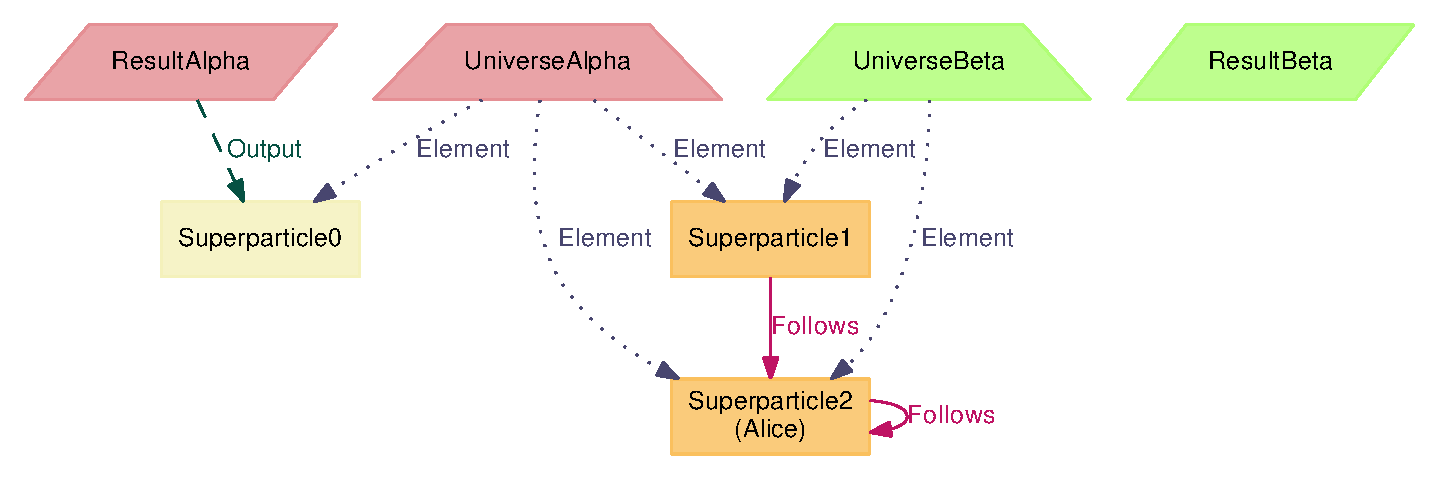
\includegraphics[width=0.99\linewidth]{figures/not-follow-alice.eps}
        \smallskip
        \caption[One counterexample of the Alloy program in \protect{\autoref{src:major-ex1}}.]{
            One counterexample of the Alloy program in \protect{\autoref{src:major-ex1}}. For an extensive explanation of this diagram, see the gray box on \hyperref[fig:not-follow-alice-exp]{page \pageref*{fig:not-follow-alice-exp}}.
        }
        \label{fig:not-follow-alice}
    % \end{mdframed}
    \vspace*{-1pc}
\end{figure}

\begin{figure}[!b]
    \begin{mdframed}[style=standard,innerbottommargin=0pc,skipabove=0pc,skipbelow=0pc]
        \ContinuedFloat
        \caption[One counterexample of the Alloy program in \protect{\autoref{src:major-ex1}}.]{
            One counterexample of the Alloy program in \protect{\autoref{src:major-ex1}}, \emph{continued from \hyperref[fig:not-follow-alice]{page \pageref*{fig:not-follow-alice}}}.

            \captionpar
            In this database model, \mbox{\textcolor[HTML]{48466f}{\dotuline{$\blacksquare$ dotted blue}}} \alloyfn{Element} arrows indicate that the first domain, \alloyfn{UniverseAlpha}, contains three scalar values whereas the second domain, \alloyfn{UniverseBeta}, has only two values (and is incidentally the subset of the first). In addition, \alloyfn{Alice} is another name for \alloyfn{Superparticle2}.

            \captionpar
            The instance of the \rel{Follows} (denoted with \mbox{\textcolor[HTML]{bf1363}{\uline{$\blacksquare$ solid pink}}} \alloyfn{Follows} arrows) contains two rows, namely
                $
                    \;\{\hrsp(\str{Superparticle1},\, \underbrace{\str{Superparticle2}}_\str{Alice}),\; (\underbrace{\str{Superparticle2}}_\str{Alice},\, \underbrace{\str{Superparticle2}}_\str{Alice})\hrsp\}
                $
            This table instance is \emph{valid} because both values \str{Superparticle1} and \str{Superparticle2} belong to \emph{both} domains.

            \captionpar
            The result of query under \alloyfn{UniverseAlpha} is a single row data $\{\str{Superparticle0}\}$ as shown by \mbox{\textcolor[HTML]{065143}{\dashuline{$\blacksquare$ dashed green}}} \alloyfn{Output} dashed arrows). On the other hand, \alloyfn{UniverseBeta} yields empty results.
        }
        \label{fig:not-follow-alice-exp}
    \end{mdframed}
    \vspace*{-1pc}
\end{figure}

\newpage
\begin{lstlisting}[language=alloy,basicstyle={\footnotesize\ttfamily},caption={The complete Alloy program which verifies the query {\protect $Q_\text{\,not\,following\,Alice}$} as shown in \autoref{ex:major-ex1}. Alloy codes highlighted in yellow indicate portions of code which are translated according to and depending on the original database schema and the \textsc{drc} query.},label={src:major-ex1},aboveskip=0pc,belowskip=0pc]
/* Scalar values */
sig Superparticle {} {
	Superparticle = Universe.Element
}

/* Domains */
abstract sig Universe { Element: some Superparticle }
one sig UniverseAlpha, UniverseBeta extends Universe {}

/* Common domain */
some sig Particle in Superparticle {} {
	Particle = UniverseAlpha.Element & UniverseBeta.Element
}

/* Database Instance */
one sig Table {
    <|\hll{ex1table}|>Follows: Particle -> Particle<|\hlr{ex1table}|>
}

/* Constant Values */
one sig Constant {
    <|\hll{ex1alice}|>Alice: Particle<|\hlr{ex1alice}\label{li:alice}|>
}

/* Lists all people who are not following Alice */
fun query[u: Universe]: <|\hll{ex1sig}|>set Superparticle<|\hlr{ex1sig}|> {
    { <|\hll{ex1x}|>x<|\hlr{ex1x}|>: u.Element | <|\hll{ex1pred}|>not (x -> Constant.Alice in Table.Follows)<|\hlr{ex1pred}\label{li:usealice}|> }
}

/* Safety assertion */
assert queryIsSafe {
    all u, u': Universe | query[u] = query[u']
}

/* Results placeholder */
abstract sig Result {
    Output: <|\hll{ex1result}|>set Superparticle<|\hlr{ex1result}|>
}
one sig ResultAlpha, ResultBeta extends Result {} {
    ResultAlpha.@Output = query[UniverseAlpha]
    ResultBeta.@Output = query[UniverseBeta]
}

/* Invoke the verification on the assertion */
check queryIsSafe for 4
\end{lstlisting}

\vspace*{3pc}
\begin{lstlisting}[language=alloy,basicstyle={\footnotesize\ttfamily},caption={The complete Alloy programw which verifies the query {\protect $Q_\text{\,follows\,all\,v2}$} as shown in \autoref{ex:major-ex2}. Alloy codes highlighted in yellow indicates portions of code which are translated according and depending on the original database schema and \textsc{drc} query. Also noted that, unlike \autoref{src:major-ex1}, this Alloy program does not require the \alloy{Constant} model.},label={src:major-ex2},aboveskip=0pc,belowskip=0pc]
/* Scalar values */
sig Superparticle {} {
	Superparticle = Universe.Element
}

/* Domains */
abstract sig Universe { Element: some Superparticle }
one sig UniverseAlpha, UniverseBeta extends Universe {}

/* Common domain */
some sig Particle in Superparticle {} {
	Particle = UniverseAlpha.Element & UniverseBeta.Element
}

/* Database Instance */ <|\label{li:ex2-replace-case1}|>
one sig Table {
    <|\hll{ex2table}|>Follows: Particle -> Particle<|\hlr{ex2table}|>
} <|\label{li:ex2-fix}|>

/* Lists all follows who follows every idols */
fun query[u: Universe]: <|\hll{ex2sig}|>set Superparticle<|\hlr{ex2sig}|> {
    { <|\hll{ex2x}|>x<|\hlr{ex2x}|>: u.Element | <|\hll{ex2pred1}|>all y: u.Element | <|\hlr{ex2pred1}\SuppressNumber|>
        <|\hll{ex2pred2}|>(some z: u.Element | z -> y in Table.Follows) <|\hlr{ex2pred2}|>
        <|\hll{ex2pred3}|>implies (x -> y in Table.Follows)<|\hlr{ex2pred3}\ReactivateNumber|> }
}

/* Safety assertion */ <|\label{li:ex2-replace-case2}|>
assert queryIsSafe {
    all u, u': Universe | query[u] = query[u']
}

/* Results placeholder */
abstract sig Result {
    Output: <|\hll{ex2result}|>set Superparticle<|\hlr{ex2result}|>
}
one sig ResultAlpha, ResultBeta extends Result {} {
    ResultAlpha.@Output = query[UniverseAlpha]
    ResultBeta.@Output = query[UniverseBeta]
}

/* Invoke the verification on the assertion */
check queryIsSafe for 4
\end{lstlisting}

\bigskip
Now let us consider another example, particularly \autoref{ex:follow-all}. In the original scenario, the query $Q_\text{\,follows\,all}$ is unsafe because the universal quantification may probe on domain values which lie outside the database. We are going to fix this query in the next example.

\newpage
\begin{example}
    \phantomsection
    \addcontentsline{toc}{subsection}{Second full example}
    \label{ex:major-ex2}
    Consider the database table $\rel{Follows}(\field{fan},\field{idol})$ and the \textsc{drc} query
    \[
        Q_\text{\,follows\,all\,v2} =
            \{ x \mid \forall y[ \exists z [\rel{Follows}(z, y)] \Rightarrow \rel{Follows}(x, y)] \}
    \]
    By additionally injecting ``$\exists z [\rel{Follows}(z, y)] \Rightarrow$'' into the original query, it \emph{hopefully} guarantees that only idols (represented by $y$) having \emph{at least} one follower in the database are considered. This should disregard the effect of dealing with different domain sets.

    We translated the database schema as well as the above query into the Alloy program as shown in \autoref{src:major-ex2}. However, once Alloy Analyzer was executed, we got unexpected results: it produces counterexamples. After a careful consideration the table \rel{Follows} in every counterexample is empty.

    \marginhead{Using Alloy to debug the query}
    Upon the second glance of the query $Q_\text{\,follows\,all\,v2}$, the result returned by Alloy Analyzer actually makes sense. If the table \rel{Follows} is empty, then the query result would be the same set of people in the domain. \emph{This is one prime example of Alloy could help us finding bugs in the design.}

    We need to fix the program to guarantee that we only considered nonempty table \rel{Follows}, which could be stated as an additional fact towards the \alloy{Table} signature declaration. Therefore, after the closing brace at the beginning of \autoref{li:ex2-fix}, we insert the fact (as highlighted) that the table \alloy{Follows} must contain some (i.e., at least one) rows.

    % FIXME USE THIS INSTEAD OF HARDCODING NUMBERS: \ref*{li:ex2-replace-case1}]}

\begin{lstlisting}[language=alloy,firstnumber=15]
/* Database Instance */
one sig Table {
    Follows: Particle -> Particle
} <|\hll{ex2fact}|>{ some Follows }<|\hlr{ex2fact}|>
\end{lstlisting}

    Once the the modified Alloy program is executed again, it no longer finds a counterexample. Even if we increase the upper limit of the number of each type of model objects from \alloy{4} to \alloy{8}, or even to \alloy{12}, Alloy still does not find a counterexample. Therefore, we may say that ``the \textsc{drc} query $Q_\text{\,follows\,all\,v2}$ \emph{could be} safe, at least as long as the table \rel{Follows} is \emph{nonempty}.''\; This is only a speculation since we could only hope that if Alloy were to find a counterexample, it should have found a small one already.

    \subsubsection*{Alternative Approach}

    Instead of checking for database instances in which the table \rel{Follows} is not empty, we could modify the query to make sure that the \field{fan} must reside in the database. Hence, let us say that the new \textsc{drc} query is
    \[
        Q_\text{\,follows\,all\,v3} =
            \{ x \mid \exists w [\rel{Follows}(x, w)] \wedge \forall y[ \exists z [\rel{Follows}(z, y)] \Rightarrow \rel{Follows}(x, y)] \}
    \]
    The first clause of the conjuction demands that the \field{fan} $x$ must follow at least one person. In other words, that \field{fan} must at least exists in the database.

    The Alloy function implementation of this query can be written as
\begin{lstlisting}[language=alloy,firstnumber=20]
/* Lists all follows who follows every idols */
fun query[u: Universe]: set Superparticle {
    { x : u.Element | <|\SuppressNumber|>
        <|\hll{ex2xtra}|>(some w: u.Element | x -> w in Table.Follows) and <|\hlr{ex2xtra}|>
        (all y: u.Element |
            (some z: u.Element | z -> y in Table.Follows)
            implies (x -> y in Table.Follows))<|\ReactivateNumber|> }
}
\end{lstlisting}
    The only difference between this new code and the original one is shown as highlighted. Everything else remains the same apart from reformatting for clarity.

    When we run this new code, the Alloy Analyzer also does not find any counterexamples, and thus the new query $Q_\text{\,follows\,all\,v3}$ may be safe.
\end{example}

Now that we have established how any simple database schemata and \textsc{drc} queries can be translated into a verification task in Alloy language, in the next section we will experiment with more examples of safe and unsafe queries and see how accurate Alloy performs the verification tasks.
